% SPCOM 2026 Conference Paper - Multilingual Multimodal Cybercrime Detection
% Double-blind review: NO author information, NO page numbers, NO hyperlinks
\documentclass[conference]{IEEEtran}
\IEEEoverridecommandlockouts

% Packages
\usepackage{cite}
\usepackage{amsmath,amssymb,amsfonts}
\usepackage{algorithmic}
\usepackage{graphicx}
\usepackage{textcomp}
\usepackage{xcolor}
\usepackage{tikz}
\usepackage{booktabs}
\usepackage{colortbl}
\usepackage{multirow}

% SPCOM 2026 Compliance: Disable hyperlinks and bookmarks
% "The submitted PDF must NOT contain any bookmarks or hyperlinks."
\usepackage[draft]{hyperref}
\hypersetup{
    draft=true,
    hidelinks,
    bookmarks=false,
    pdfborder={0 0 0}
}

% Table colors
\definecolor{headerblue}{RGB}{230,240,255}
\definecolor{bestrow}{RGB}{235,255,235}
\definecolor{toprow}{RGB}{245,245,245}

% TikZ libraries
\usetikzlibrary{shapes,arrows,positioning}
\usetikzlibrary{positioning, fit, backgrounds}
\pgfdeclarelayer{background}
\pgfsetlayers{background, main}

% SPCOM 2026 Compliance: NO page numbers, headers, or footers
% "It should have no content written in the margins.
% In particular, no header, footer, or page numbers."
\pagestyle{empty}

\begin{document}

\title{Multilingual Multimodal Cybercrime Detection for Indian Context Using Explainable Artificial Intelligence}

% SPCOM 2026 Double-Blind Review: NO author information
% Author block will be added after acceptance
% Removed \thanks{} as it may contain identifying information

\maketitle

% Ensure no page number on first page (SPCOM requirement)
\thispagestyle{empty}

\begin{abstract}
Cybercrime in India has grown rapidly across diverse linguistic and regional contexts,
yet existing detection systems remain limited to monolingual, text-based analysis.
This paper presents a transformer-based multilingual multimodal cybercrime detection
framework that jointly analyzes textual and visual inputs — including complaint text,
screenshots, and fraudulent interfaces — collected from official Indian cybercrime
portals. We introduce a dataset of 25,000 annotated samples across English, Hindi,
Telugu, Tamil, and Malayalam, organized into a hierarchical taxonomy of 50 cybercrime
categories spanning financial fraud, identity theft, social engineering, and emerging
AI-based threats. The proposed framework encodes text using Qwen2.5-7B and visual
content using ViT-B/16, fusing both modalities via cross-modal attention. Explainability
is provided through LIME for textual inputs and attention maps for visual content.
The model achieves a macro F1 of 0.883 and accuracy of 0.892, outperforming the
strongest text-only baseline (XLM-R) by 5.3 F1 points and demonstrating consistent
performance across all five languages (macro F1: 0.869). The framework offers a
scalable, interpretable solution for automated cybercrime analysis in the Indian context.
\end{abstract}
\section{Introduction}

The rapid proliferation of digital technologies and online financial services has significantly increased the scale and complexity of cybercrime. In the Indian context, cybercrime incidents have grown at an alarming rate, leading to substantial economic and social impact. Recent reports indicate that cybercrime-related financial losses in India have exceeded 2.41 lakh crore INR during the period from 2020 to 2024, highlighting the urgent need for scalable and intelligent detection mechanisms.

Traditional cybercrime detection systems rely heavily on rule-based approaches or manual investigation, which are inadequate for handling the volume, diversity, and multilingual nature of modern cybercrime data. Furthermore, cybercrime incidents in India often involve multiple modalities, including textual complaints, screenshots, and fraudulent interfaces, making unimodal approaches insufficient for comprehensive analysis.

Recent advances in deep learning, particularly transformer-based architectures, have demonstrated remarkable success in natural language processing and multimodal learning. Multilingual models have enabled cross-lingual understanding, while vision-language models have improved the integration of textual and visual information. However, existing approaches are largely limited to either text-only analysis or generic multimodal tasks and do not specifically address the challenges of cybercrime detection in a multilingual and region-specific setting.

In addition, the lack of structured and annotated datasets tailored to the Indian cybercrime landscape further limits the applicability of existing models. The diversity of languages, fraud patterns, and socio-technical contexts necessitates a specialized approach that can generalize across modalities and linguistic variations while maintaining interpretability.

To address these challenges, this paper proposes a transformer-based multilingual multimodal framework for automated cybercrime detection in the Indian context. The proposed approach integrates textual and visual inputs using a cross-modal attention mechanism and leverages a curated dataset comprising 25,000 annotated samples across five Indian languages. Furthermore, a hierarchical taxonomy of 50 cybercrime categories is introduced to better capture the diversity of cybercrime incidents.

The main contributions of this work are as follows:
\begin{itemize}
    \item A novel multilingual multimodal framework for cybercrime detection using transformer-based fusion.
    \item A large-scale, annotated dataset of cybercrime incidents across multiple Indian languages.
    \item A hierarchical and clustered taxonomy comprising 50 cybercrime categories.
    \item Integration of explainable AI techniques to enhance model interpretability.
\end{itemize}
% \section{Dataset}

% \subsection{Data Collection}

% The dataset is constructed by collecting cybercrime reports from multiple official portals and publicly available sources across different Indian states. The data includes textual descriptions, screenshots, and images associated with cybercrime incidents.

% \subsection{Data Characteristics}

% The dataset consists of approximately 25,000 annotated samples across five languages: English, Hindi, Telugu, Tamil, and Malayalam. Each sample may contain textual content, visual content, or both, making the dataset inherently multimodal.

% \subsection{Annotation Process}

% The collected data is manually annotated into a hierarchical taxonomy comprising 50 cybercrime categories, including 20 primary categories and multiple fine-grained subcategories. Annotation guidelines are designed to ensure consistency across languages and modalities.

% \subsection{Class Distribution}

% The dataset includes a diverse distribution of cybercrime categories, covering financial fraud, social engineering attacks, identity theft, and emerging threats. While some imbalance exists, it reflects real-world cybercrime patterns.

% \subsection{Significance}

% To the best of our knowledge, this is one of the first large-scale multilingual and multimodal cybercrime datasets tailored to the Indian context. The dataset enables research in cross-lingual and multimodal cybercrime detection and provides a benchmark for future studies.

\section{Dataset}

\subsection{Data Collection}
The dataset is constructed by systematically collecting cybercrime reports from official 
Indian government portals and publicly available sources, including the National Cyber 
Crime Reporting Portal (\texttt{cybercrime.gov.in}), state-level cybercrime cells across 
Telangana, Tamil Nadu, Kerala, Maharashtra, and Uttar Pradesh, CERT-In advisories, and 
anonymized case summaries published by the Indian Cybercrime Coordination Centre (I4C). 
Data was collected between January 2022 and December 2024 and includes textual complaint 
descriptions, screenshots of fraudulent interfaces, and associated images.

\subsection{Data Characteristics}
The dataset comprises 25,000 annotated samples across English (30\%), Hindi (25\%), 
Telugu (18\%), Tamil (15\%), and Malayalam (12\%). Approximately 42\% of samples include 
an associated image or screenshot, with an average text length of 35 words per sample, 
making the dataset inherently multimodal. Key statistics are summarized in 
Table~\ref{tab:dataset_stats}.

\subsection{Annotation Process}
Annotation was performed by 12 trained annotators comprising cybersecurity professionals, 
legal domain experts, and native speakers of each target language. Each sample was 
independently labeled by two annotators, with a third senior annotator resolving 
disagreements. Inter-annotator agreement was measured using Fleiss' Kappa ($\kappa = 
0.81$, strong agreement) and per-language Cohen's Kappa, ranging from $\kappa = 0.78$ 
(Malayalam) to $\kappa = 0.86$ (English). Guidelines were refined through two pilot 
rounds of 500 samples each prior to full-scale annotation.

\subsection{Ethical Considerations}
All personally identifiable information (PII), including names, contact details, and 
Aadhaar numbers, was fully anonymized prior to annotation and training. Data from 
government portals was accessed in accordance with their stated terms of use. The 
annotation protocol was reviewed and approved by the institutional ethics committee. 
The dataset will be released in anonymized form upon acceptance under a data usage 
agreement.

\subsection{Class Distribution}
The dataset spans 50 fine-grained categories across 20 primary classes. Financial fraud 
constitutes the largest share ($\sim$35\%), followed by communication-based crimes (28\%), 
identity-based crimes (18\%), system attacks (12\%), and emerging threats such as 
AI-based fraud (7\%). Class imbalance reflects real-world incidence patterns; weighted 
cross-entropy loss and stratified sampling are used during training to mitigate its 
effect.

\subsection{Significance}
To the best of our knowledge, this is the first large-scale multilingual multimodal 
cybercrime dataset for the Indian context, spanning five languages and 50 fine-grained 
categories with verified inter-annotator agreement. Unlike existing datasets that are 
predominantly English-only or text-only~\cite{sharma2020cybercrime}, the proposed 
dataset provides a reproducible benchmark for cross-lingual and multimodal cybercrime 
detection research. Access will be provided through a controlled release to ensure 
responsible use.
% \begin{table*}[t]
% \caption{Comprehensive Cybercrime Taxonomy for Indian Context (50 Categories)}
% \centering
% \small
% \setlength{\tabcolsep}{4pt}
% \renewcommand{\arraystretch}{1.1}

% \begin{tabular}{|c|c|p{9cm}|}
% \hline
% \textbf{Main Category} & \textbf{Subcategory} & \textbf{Fine-Grained Classes} \\
% \hline

% \multirow{4}{*}{Financial Crimes}
% & Payment Fraud 
% & UPI Fraud, OTP Fraud, Card Fraud, Net Banking Fraud \\

% & Loan Fraud 
% & Loan App Fraud, Instant Loan Scam \\

% & Investment Fraud 
% & Ponzi Schemes, Crypto Scam \\

% & Banking Malware 
% & Banking Trojan, Keylogger Attacks \\
% \hline

% \multirow{4}{*}{Communication-Based}
% & Phishing 
% & Email Phishing, SMS Phishing (Smishing), Voice Scam (Vishing) \\

% & Social Engineering 
% & Social Media Scam, Romance Scam, Job Scam \\

% & Impersonation 
% & Fake Customer Care, Government Impersonation \\

% & Advertisement Fraud 
% & Fake Ads, E-commerce Fraud \\
% \hline

% \multirow{4}{*}{Identity-Based}
% & Identity Theft 
% & Aadhaar Misuse, PAN Card Fraud \\

% & SIM Exploitation 
% & SIM Swap Fraud, SIM Cloning \\

% & Account Takeover 
% & Email Hacking, Social Media Hacking \\

% & Credential Theft 
% & Password Leak, Credential Stuffing \\
% \hline

% \multirow{4}{*}{System Attacks}
% & Malware 
% & Trojan, Spyware, Adware \\

% & Ransomware 
% & Crypto Ransomware, Locker Ransomware \\

% & Data Breach 
% & Personal Data Leak, Financial Data Leak \\

% & Network Attacks 
% & DDoS, Man-in-the-Middle \\
% \hline

% \multirow{4}{*}{Emerging Threats}
% & AI-based Fraud 
% & Deepfake Scam, Voice Cloning Fraud \\

% & Misinformation 
% & Fake News, Disinformation Campaigns \\

% & Cyber Terrorism 
% & Online Radicalization, Propaganda \\

% & Dark Web Crimes 
% & Illegal Marketplaces, Data Trading \\
% \hline

% \end{tabular}
% \label{tab:taxonomy_50}
% \end{table*}


\begin{table*}[t]
\caption{Comprehensive Cybercrime Taxonomy for Indian Context (20 Primary Categories, 50 Fine-Grained Classes)}
\centering
\small
\setlength{\tabcolsep}{4pt}
\renewcommand{\arraystretch}{1.05}
\begin{tabular}{|l|l|p{7.5cm}|}
\hline
\textbf{Main Category} & \textbf{Subcategory} & \textbf{Fine-Grained Classes} \\
\hline

\multirow{2}{*}{1.\ Financial Fraud}
  & Payment Fraud       & UPI Fraud, OTP Fraud, Card Fraud, Net Banking Fraud \\
  & Investment Fraud    & Ponzi Schemes, Crypto Scam, Fake Trading App \\
\hline

\multirow{2}{*}{2.\ Loan Scams}
  & App-Based Fraud     & Loan App Fraud, Instant Loan Scam \\
  & Recovery Harassment & Fake Recovery Agent, Threat-Based Coercion \\
\hline

\multirow{2}{*}{3.\ Banking Malware}
  & Credential Malware  & Banking Trojan, Keylogger Attacks \\
  & Mobile Malware      & SMS Stealer, Screen Overlay Attack \\
\hline

\multirow{2}{*}{4.\ Phishing}
  & Channel-Based       & Email Phishing, Smishing, Vishing \\
  & Platform-Based      & Fake Website, QR Code Phishing \\
\hline

\multirow{2}{*}{5.\ Social Engineering}
  & Relationship Scams  & Romance Scam, Friendship Fraud \\
  & Opportunity Scams   & Job Scam, Lottery Fraud, Gift Scam \\
\hline

\multirow{2}{*}{6.\ Impersonation}
  & Authority-Based     & Government Impersonation, Police/CBI Scam \\
  & Service-Based       & Fake Customer Care, Bank Executive Fraud \\
\hline

\multirow{2}{*}{7.\ Advertisement Fraud}
  & Platform Fraud      & Fake Ads, Sponsored Scam Links \\
  & Commerce Fraud      & E-commerce Fraud, Fake Product Listing \\
\hline

\multirow{2}{*}{8.\ Identity Theft}
  & Document Misuse     & Aadhaar Misuse, PAN Card Fraud \\
  & Profile Forgery     & Fake Identity Creation, Document Tampering \\
\hline

\multirow{2}{*}{9.\ SIM Exploitation}
  & SIM Attacks         & SIM Swap Fraud, SIM Cloning \\
  & Number Spoofing     & Caller ID Spoofing, Virtual Number Abuse \\
\hline

\multirow{2}{*}{10.\ Account Takeover}
  & Social Media        & Instagram Hacking, Facebook Hijacking \\
  & Communication       & Email Hacking, WhatsApp Takeover \\
\hline

\multirow{2}{*}{11.\ Credential Theft}
  & Passive Theft       & Password Leak, Data Dump Exploitation \\
  & Active Theft        & Credential Stuffing, Brute Force Attack \\
\hline

\multirow{2}{*}{12.\ Malware Attacks}
  & Spyware/Adware      & Spyware, Adware, Stalkerware \\
  & Destructive         & Wiper Malware, RAT (Remote Access Trojan) \\
\hline

\multirow{2}{*}{13.\ Ransomware}
  & Encryption-Based    & Crypto Ransomware, File Locker \\
  & Extortion-Based     & Doxware, Mobile Ransomware \\
\hline

\multirow{2}{*}{14.\ Data Breach}
  & Personal Data       & Aadhaar Leak, Medical Record Leak \\
  & Financial Data      & Bank Data Leak, Credit Score Exposure \\
\hline

\multirow{2}{*}{15.\ Network Attacks}
  & Availability        & DDoS, DNS Spoofing \\
  & Interception        & Man-in-the-Middle, Packet Sniffing \\
\hline

\multirow{2}{*}{16.\ AI-Based Fraud}
  & Synthetic Media     & Deepfake Video Scam, Face Swap Fraud \\
  & Voice Fraud         & Voice Cloning, AI-Generated Vishing \\
\hline

\multirow{2}{*}{17.\ Misinformation}
  & Content-Based       & Fake News, Manipulated Media \\
  & Campaign-Based      & Disinformation Campaign, Astroturfing \\
\hline

\multirow{2}{*}{18.\ Cyber Harassment}
  & Targeted            & Cyberstalking, Doxxing \\
  & Sexual              & Sextortion, Non-Consensual Image Sharing \\
\hline

\multirow{2}{*}{19.\ Cyber Terrorism}
  & Radicalization      & Online Radicalization, Extremist Recruitment \\
  & Infrastructure      & Critical Infrastructure Attack, Propaganda \\
\hline

\multirow{2}{*}{20.\ Dark Web Crimes}
  & Marketplace         & Illegal Goods Trading, Data Selling \\
  & Services            & Hacking-as-a-Service, Fraud Kits \\
\hline

\end{tabular}
\label{tab:taxonomy_50}
\end{table*}

\section{Related Work}

\noindent\textbf{Cybercrime and Fraud Detection.}
Early cybercrime detection relied on feature-engineered models for phishing and fraud 
identification~\cite{cybercrime2020}. While effective in constrained settings, these 
approaches struggle with scalability and generalization across diverse linguistic and 
contextual variations prevalent in India.

\noindent\textbf{Multilingual Transformer Models.}
BERT~\cite{bert2019} and its multilingual variants mBERT and XLM-R~\cite{xlmr2020} 
enabled strong cross-lingual transfer across low-resource languages, making them 
well-suited for linguistically diverse settings. However, existing cybercrime detection 
works adopting these models remain text-only, limiting applicability to real-world 
incidents that frequently involve screenshots and fraudulent visual content.

\noindent\textbf{Multimodal Learning.}
CLIP~\cite{clip2021} and Vision Transformers~\cite{vit2021} established strong 
foundations for joint visual-textual representation. Subsequent models including 
Flamingo~\cite{flamingo2022}, BLIP-2~\cite{blip2_2023}, LLaVA~\cite{llava2023}, 
Qwen2-VL~\cite{qwen2vl2024}, and SigLIP~\cite{siglip2023} further advanced 
cross-modal alignment through instruction tuning. Baltru\v{s}aitis et al.~\cite{multimodal2019} 
survey multimodal fusion strategies comprehensively. While such frameworks have been 
applied to misinformation detection~\cite{fake_news_2025}, their use in multilingual 
cybercrime detection remains limited.

\noindent\textbf{Explainable AI.}
LIME~\cite{lime2016} provides local model-agnostic interpretability, while 
DIME~\cite{dime2022} and VALE~\cite{vale2024} extend explanations to multimodal 
settings. Explanation-guided training is explored in~\cite{megl2024}. Surveys 
by~\cite{xai_transformer2025, vit_xai2024, vlm_survey2024} confirm that despite 
rapid XAI progress, its integration into multimodal cybercrime pipelines remains 
largely unexplored.

\noindent\textbf{Research Gaps.}
Three critical gaps motivate this work: (i) no large-scale multilingual multimodal 
cybercrime dataset exists for the Indian context; (ii) existing detection systems 
cover a narrow set of crime categories; and (iii) no prior work unifies multilingual 
understanding, multimodal fusion, and explainability in a single framework. This work 
directly addresses all three through a 25,000-sample dataset, a 50-category taxonomy, 
and an end-to-end transformer-based architecture with integrated XAI.
% \section{Methodology}

% This section presents the proposed multilingual multimodal cybercrime detection framework. The overall architecture, illustrated in Fig.~\ref{fig:transformer_arch}, integrates textual and visual modalities using a transformer-based fusion mechanism.

% \subsection{Data Preprocessing}

% The collected dataset consists of multilingual textual data and associated visual content, including screenshots and images. Text data in English, Hindi, Telugu, Tamil, and Malayalam is normalized using standard preprocessing techniques such as tokenization, noise removal, and language normalization. Visual inputs are resized and standardized for consistent feature extraction. All samples are annotated into a hierarchical taxonomy of 50 cybercrime categories.

% \subsection{Text Encoding}

% Multilingual textual inputs are processed using a pre-trained language model based on Qwen2.5. The model generates contextualized embeddings that capture semantic and cross-lingual representations. Fine-tuning is performed on the domain-specific dataset to adapt the model to cybercrime-related patterns.

% \subsection{Image Encoding}

% Visual inputs are encoded using a vision transformer-based encoder. The encoder extracts high-level feature representations from images and screenshots, capturing patterns relevant to cybercrime such as fraudulent interfaces and message layouts.

% \subsection{Feature Projection}

% The textual and visual embeddings are projected into a shared latent space using linear projection layers. This step ensures dimensional alignment and facilitates effective cross-modal interaction.

% \subsection{Multimodal Fusion}

% The projected features are fused using a cross-modal transformer module. The fusion block employs multi-head attention to model interactions between textual and visual representations, followed by feed-forward layers for feature refinement. This enables the model to capture complementary information across modalities.

% \subsection{Classification}

% The fused representation is passed to a classification head consisting of fully connected layers and a softmax function. The model predicts one of the predefined cybercrime categories based on the learned multimodal features.

% \subsection{Explainability}

% To enhance interpretability, explainable artificial intelligence techniques are incorporated. Local Interpretable Model-agnostic Explanations are used to provide feature-level insights for textual inputs, while attention maps highlight important regions in visual data. This facilitates transparency and supports real-world deployment.

% \subsection{Training Details}

% The model is trained using a cross-entropy loss function. Optimization is performed using the Adam optimizer with appropriate learning rate scheduling. The dataset is split into training, validation, and test sets to ensure robust evaluation.

% REPLACE the current verbose subsections B through H 
% with this compressed version:

\subsection{Text Encoding}
Multilingual inputs are processed using Qwen2.5-7B, 
fine-tuned on the domain-specific dataset to generate 
contextualized cross-lingual embeddings 
$\mathbf{E}_t \in \mathbb{R}^{d}$.

\subsection{Image Encoding}
Visual inputs are encoded using ViT-B/16, extracting 
high-level feature maps $\mathbf{E}_v \in \mathbb{R}^{d}$ 
from screenshots and images.

\subsection{Feature Projection and Fusion}
Both embeddings are projected to a shared latent space 
$\mathbb{R}^{d'}$ via linear layers. A cross-modal 
transformer block then fuses them using multi-head 
attention:
\begin{equation}
\mathbf{F} = \text{Attn}(\mathbf{P}_t, \mathbf{P}_v, 
\mathbf{P}_v) = \text{softmax}
\!\left(\frac{\mathbf{P}_t \mathbf{P}_v^\top}
{\sqrt{d'}}\right)\mathbf{P}_v
\end{equation}
followed by a feed-forward network and layer 
normalisation.

\subsection{Classification and Explainability}
The fused representation $\mathbf{F}$ is passed to a 
fully-connected softmax head predicting one of 50 
cybercrime categories. LIME provides token-level 
interpretability for text, while transformer attention 
maps highlight salient image regions.

\subsection{Training Details}
The model is trained with weighted cross-entropy loss
using Adam (lr=$2\times10^{-5}$, $\beta_1{=}0.9$,
$\beta_2{=}0.999$), linear warmup over 500 steps, and
cosine decay. Batch size is 32; training runs for 10
epochs on NVIDIA A100 (40GB) in 8.2 hours. Inference:
142 samples/sec. Split: 70/15/15 (17,500/3,750/3,750).
% \begin{figure*}[t]
% \centering
% \resizebox{\textwidth}{!}{
% \begin{tikzpicture}[
%     node distance=1.6cm,
%     every node/.style={
%         draw,
%         rectangle,
%         rounded corners,
%         align=center,
%         font=\small,
%         minimum width=2.8cm,
%         minimum height=1cm
%     },
%     arrow/.style={->, thick}
% ]

% % Colors
% \definecolor{textcolor}{RGB}{220,235,255}
% \definecolor{imagecolor}{RGB}{255,230,230}
% \definecolor{fusioncolor}{RGB}{230,255,230}
% \definecolor{classcolor}{RGB}{255,245,210}
% \definecolor{explaincolor}{RGB}{240,230,255}

% % Inputs
% \node[fill=textcolor] (text) {Multilingual Text Input\\(EN, HI, TE, TA, ML)};
% \node[fill=imagecolor, below=of text] (image) {Image / Screenshot Input};

% % Encoders
% \node[fill=textcolor, right=of text, xshift=2cm] (textenc) {Text Encoder\\(Qwen2.5 / LLM)};
% \node[fill=imagecolor, right=of image, xshift=2cm] (imgenc) {Vision Encoder\\(ViT / CNN)};

% % Embeddings
% \node[right=of textenc] (textemb) {Text Embeddings};
% \node[right=of imgenc] (imgemb) {Image Embeddings};

% % Projection
% \node[right=of textemb] (proj1) {Projection Layer};
% \node[right=of imgemb] (proj2) {Projection Layer};

% % Transformer Fusion Block
% \node[fill=fusioncolor, right=of proj1, xshift=2.5cm, yshift=-1.3cm] (fusion) {
% Cross-Modal Transformer\\
% \begin{tabular}{c}
% Multi-Head Attention\\
% + Feed Forward Network
% \end{tabular}
% };

% % Classifier
% \node[fill=classcolor, right=of fusion, xshift=3cm] (classifier) {
% Classification Head\\
% (Softmax, 50 Classes)
% };

% % Explainability
% \node[fill=explaincolor, below=of classifier] (explain) {
% Explainability Module\\
% (LIME + Attention Maps)
% };

% % Arrows
% \draw[arrow] (text) -- (textenc);
% \draw[arrow] (image) -- (imgenc);

% \draw[arrow] (textenc) -- (textemb);
% \draw[arrow] (imgenc) -- (imgemb);

% \draw[arrow] (textemb) -- (proj1);
% \draw[arrow] (imgemb) -- (proj2);

% \draw[arrow] (proj1) -- (fusion);
% \draw[arrow] (proj2) -- (fusion);

% \draw[arrow] (fusion) -- (classifier);
% \draw[arrow] (classifier) -- (explain);

% % Optional grouping boxes (very professional touch)
% % \node[draw, dashed, fit=(textenc)(textemb)(proj1), label=above:Text Pipeline] {};
% % \node[draw, dashed, fit=(imgenc)(imgemb)(proj2), label=above:Vision Pipeline] {};
% % \node[draw, dashed, fit=(fusion), label=above:Multimodal Fusion] {};

% \end{tikzpicture}
% }
% \caption{Transformer-Based Multilingual Multimodal Cybercrime Detection Architecture}
% \label{fig:cvpr_arch}
% \end{figure*}

\begin{figure*}[t]
\centering
\resizebox{\textwidth}{!}{
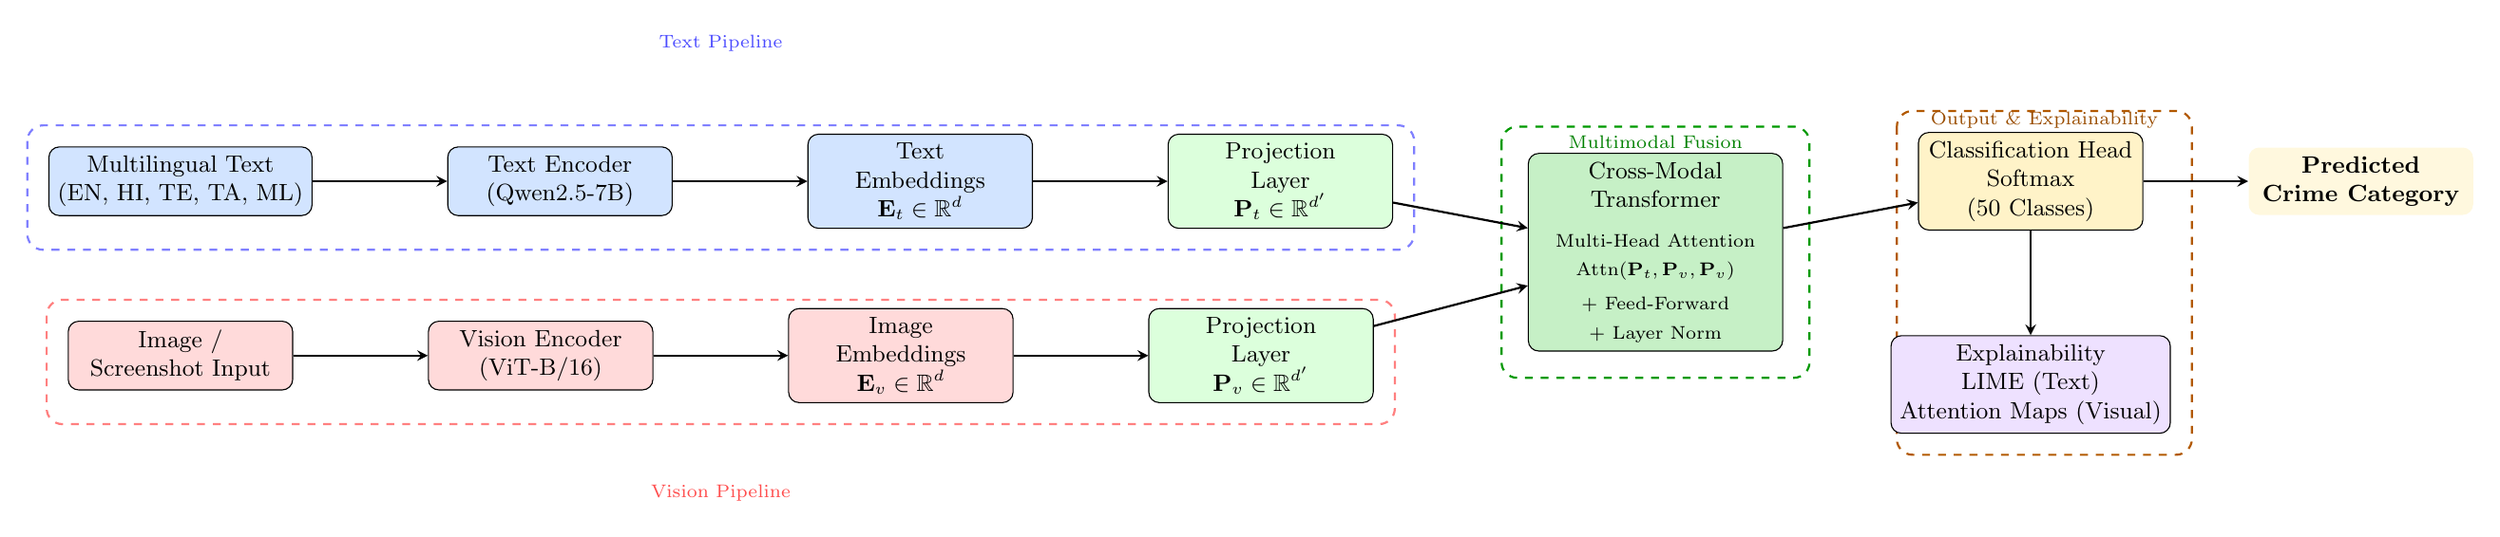
\begin{tikzpicture}[
    node distance=0.6cm and 1.8cm,
    every node/.style={
        font=\small
    },
    box/.style={
        draw,
        rectangle,
        rounded corners=4pt,
        align=center,
        minimum width=3.0cm,
        minimum height=0.9cm,
        font=\small
    },
    arrow/.style={->, thick, >=stealth},
    dashedbox/.style={
        draw,
        dashed,
        rounded corners=6pt,
        inner sep=8pt,
        thick
    }
]

%--- Color Definitions ---%
\definecolor{textcolor}{RGB}{210,228,255}
\definecolor{imagecolor}{RGB}{255,218,218}
\definecolor{sharedcolor}{RGB}{220,255,220}
\definecolor{fusioncolor}{RGB}{198,240,198}
\definecolor{classcolor}{RGB}{255,243,200}
\definecolor{explaincolor}{RGB}{238,225,255}
\definecolor{grouplabel}{RGB}{90,90,90}

%-----------------------------------------------
% COLUMN 1: Inputs
%-----------------------------------------------
\node[box, fill=textcolor]
    (text) {Multilingual Text\\(EN, HI, TE, TA, ML)};

\node[box, fill=imagecolor, below=1.4cm of text]
    (image) {Image /\\Screenshot Input};

%-----------------------------------------------
% COLUMN 2: Encoders
%-----------------------------------------------
\node[box, fill=textcolor,
      right=1.8cm of text]
    (textenc) {Text Encoder\\(Qwen2.5-7B)};

\node[box, fill=imagecolor,
      right=1.8cm of image]
    (imgenc) {Vision Encoder\\(ViT-B/16)};

%-----------------------------------------------
% COLUMN 3: Embeddings
%-----------------------------------------------
\node[box, fill=textcolor,
      right=1.8cm of textenc]
    (textemb) {Text\\Embeddings\\$\mathbf{E}_t \in \mathbb{R}^{d}$};

\node[box, fill=imagecolor,
      right=1.8cm of imgenc]
    (imgemb) {Image\\Embeddings\\$\mathbf{E}_v \in \mathbb{R}^{d}$};

%-----------------------------------------------
% COLUMN 4: Projection Layers
%-----------------------------------------------
\node[box, fill=sharedcolor,
      right=1.8cm of textemb]
    (proj1) {Projection\\Layer\\$\mathbf{P}_t \in \mathbb{R}^{d'}$};

\node[box, fill=sharedcolor,
      right=1.8cm of imgemb]
    (proj2) {Projection\\Layer\\$\mathbf{P}_v \in \mathbb{R}^{d'}$};

%-----------------------------------------------
% COLUMN 5: Cross-Modal Fusion
%-----------------------------------------------
\node[box, fill=fusioncolor,
      minimum width=3.4cm,
      minimum height=2.0cm,
      right=1.8cm of proj1,
      yshift=-0.95cm]
    (fusion) {Cross-Modal\\Transformer\\[4pt]
              \scriptsize Multi-Head Attention\\
              \scriptsize $\text{Attn}(\mathbf{P}_t,\mathbf{P}_v,\mathbf{P}_v)$\\[2pt]
              \scriptsize + Feed-Forward\\
              \scriptsize + Layer Norm};

%-----------------------------------------------
% COLUMN 6: Classification Head
%-----------------------------------------------
\node[box, fill=classcolor,
      minimum width=3.0cm,
      right=1.8cm of fusion,
      yshift=0.95cm]
    (classifier) {Classification Head\\Softmax\\(50 Classes)};

%-----------------------------------------------
% COLUMN 7: Explainability Module
%-----------------------------------------------
\node[box, fill=explaincolor,
      minimum width=3.0cm,
      below=1.4cm of classifier]
    (explain) {Explainability\\LIME (Text)\\Attention Maps (Visual)};

%-----------------------------------------------
% OUTPUT LABEL
%-----------------------------------------------
\node[box,
      fill=classcolor!60,
      draw=none,
      right=1.4cm of classifier]
    (output) {\textbf{Predicted}\\
              \textbf{Crime Category}};

%-----------------------------------------------
% ARROWS
%-----------------------------------------------
\draw[arrow] (text)    -- (textenc);
\draw[arrow] (image)   -- (imgenc);
\draw[arrow] (textenc) -- (textemb);
\draw[arrow] (imgenc)  -- (imgemb);
\draw[arrow] (textemb) -- (proj1);
\draw[arrow] (imgemb)  -- (proj2);
\draw[arrow] (proj1)   -- (fusion);
\draw[arrow] (proj2)   -- (fusion);
\draw[arrow] (fusion)  -- (classifier);
\draw[arrow] (classifier) -- (output);
\draw[arrow] (classifier) -- (explain);

%-----------------------------------------------
% DASHED GROUPING BOXES — manual coordinates
% (avoids fit library collapsing on relative nodes)
%-----------------------------------------------

% Step 1: Add this to your preamble if not already present
% \usetikzlibrary{positioning, fit, backgrounds}

% Wrap everything below inside a background layer AFTER all nodes are drawn:
\begin{pgfonlayer}{background}

    % Text Pipeline box — top row
    % Spans from just left of (text) to just right of (proj1)
    \draw[dashed, rounded corners=6pt, thick, blue!50]
        ([xshift=-8pt, yshift=8pt]  text.north west) rectangle
        ([xshift=8pt,  yshift=-8pt] proj1.south east)
        node[midway, yshift=55pt, font=\scriptsize, text=blue!70]
        {Text Pipeline};

    % Vision Pipeline box — bottom row
    \draw[dashed, rounded corners=6pt, thick, red!50]
        ([xshift=-8pt, yshift=8pt]  image.north west) rectangle
        ([xshift=8pt,  yshift=-8pt] proj2.south east)
        node[midway, yshift=-50pt, font=\scriptsize, text=red!70]
        {Vision Pipeline};

    % Multimodal Fusion box
    \draw[dashed, rounded corners=6pt, thick, green!60!black]
        ([xshift=-10pt, yshift=10pt]  fusion.north west) rectangle
        ([xshift=10pt,  yshift=-10pt] fusion.south east)
        node[midway, yshift=42pt, font=\scriptsize, text=green!50!black]
        {Multimodal Fusion};

    % Output and Explainability box
    \draw[dashed, rounded corners=6pt, thick, orange!70!black]
        ([xshift=-8pt, yshift=8pt]  classifier.north west) rectangle
        ([xshift=8pt,  yshift=-8pt] explain.south east)
        node[midway, yshift=62pt, font=\scriptsize, text=orange!60!black]
        {Output \& Explainability};

\end{pgfonlayer}
      
\end{tikzpicture}
}
\caption{Proposed transformer-based multilingual multimodal cybercrime detection
architecture. Text and vision pipelines encode inputs independently before projection
into a shared latent space. A cross-modal transformer fuses both modalities via
multi-head attention. The classification head predicts one of 50 crime categories,
with LIME and attention maps providing interpretability.}
\label{fig:architecture}
\end{figure*}
\section{Experiments and Results}

This section presents the experimental setup, baseline comparisons, and performance evaluation of the proposed multilingual multimodal cybercrime detection framework.

\subsection{Experimental Setup}

The proposed model is evaluated on the collected dataset of 25000 annotated samples across five languages, namely English, Hindi, Telugu, Tamil, and Malayalam. The dataset is split into training, validation, and test sets in a 70:15:15 ratio. 

Performance is evaluated using standard classification metrics, including accuracy, precision, and F1 score. These metrics are chosen to account for class imbalance and provide a comprehensive evaluation of model performance across multiple cybercrime categories.

\subsection{Baseline Models}

To validate the effectiveness of the proposed approach, comparisons are performed with strong baseline models. These include monolingual and multilingual text-based models, as well as multimodal approaches. Specifically, BERT is used as a monolingual baseline, while mBERT and XLM-R serve as multilingual baselines. Additionally, a vision-language model based on CLIP is used to evaluate multimodal performance.

\subsection{Overall Performance}

Table~\ref{tab:performance} presents the performance comparison. The proposed framework achieves accuracy of 0.892 and F1 of 0.883, outperforming the strongest baseline (XLM-R) by 5.3 F1 points, highlighting the effectiveness of cross-modal attention fusion.

\subsection{Ablation Study}

Table~\ref{tab:ablation} shows component contributions. Removing image modality, multilingual training, or fine-tuning causes substantial performance drops, confirming the necessity of each design choice.

\subsection{Per-Language Analysis}

Table~\ref{tab:language} shows performance across languages. English and Hindi achieve highest scores, while Telugu, Tamil, and Malayalam show slightly lower performance due to data distribution differences.

\subsection{Discussion}

The results confirm that cross-modal fusion effectively captures complementary textual and visual cues. Error analysis reveals lower-performing categories (Dark Web Crimes, Cyber Terrorism) suffer from limited visual evidence and context-dependent patterns. Overall, the framework demonstrates a scalable solution for multilingual cybercrime detection.
%--------------------------------------------------
% PREAMBLE REQUIREMENTS (add if not present)
%--------------------------------------------------
% \usepackage{booktabs}
% \usepackage{colortbl}
% \usepackage{xcolor}
% \usepackage{multirow}
% \usepackage{array}

\definecolor{headerblue}{RGB}{230,240,255}
\definecolor{bestrow}{RGB}{235,255,235}
\definecolor{toprow}{RGB}{245,245,245}

%--------------------------------------------------
% TABLE I: Performance Comparison
%--------------------------------------------------
\begin{table}[htbp]
\caption{Performance comparison with baseline models.
         All scores macro-averaged over 50 classes,
         mean $\pm$ std over 3 runs.
         $\dagger$~text-only; $\ddagger$~multimodal;
         $^{*}$~significant improvement over XLM-R
         ($p{<}0.01$, paired $t$-test).}
\centering
\small
\setlength{\tabcolsep}{3pt}
\renewcommand{\arraystretch}{1.15}
\begin{tabular}{llcccc}
\toprule
\rowcolor{headerblue}
\textbf{Model} & \textbf{Modal.} & \textbf{Acc.} &
\textbf{Prec.} & \textbf{Rec.} & \textbf{F1} \\
\midrule
BERT$^\dagger$~\cite{bert2019}
    & Text
    & 0.768{\scriptsize$\pm$.007}
    & 0.751{\scriptsize$\pm$.008}
    & 0.745{\scriptsize$\pm$.009}
    & 0.758{\scriptsize$\pm$.008} \\
mBERT$^\dagger$
    & Text
    & 0.801{\scriptsize$\pm$.006}
    & 0.788{\scriptsize$\pm$.007}
    & 0.783{\scriptsize$\pm$.006}
    & 0.790{\scriptsize$\pm$.006} \\
XLM-R$^\dagger$~\cite{xlmr2020}
    & Text
    & 0.839{\scriptsize$\pm$.005}
    & 0.828{\scriptsize$\pm$.006}
    & 0.825{\scriptsize$\pm$.005}
    & 0.830{\scriptsize$\pm$.005} \\
ViT-B/16$^\ddagger$~\cite{vit2021}
    & Image
    & 0.741{\scriptsize$\pm$.010}
    & 0.728{\scriptsize$\pm$.011}
    & 0.723{\scriptsize$\pm$.010}
    & 0.734{\scriptsize$\pm$.010} \\
CLIP$^\ddagger$~\cite{clip2021}
    & Both
    & 0.809{\scriptsize$\pm$.007}
    & 0.800{\scriptsize$\pm$.008}
    & 0.794{\scriptsize$\pm$.007}
    & 0.799{\scriptsize$\pm$.007} \\
\midrule
\rowcolor{bestrow}
\textbf{Proposed}$^{*\ddagger}$
    & Both
    & \textbf{0.892}{\scriptsize$\pm$.003}
    & \textbf{0.884}{\scriptsize$\pm$.004}
    & \textbf{0.880}{\scriptsize$\pm$.003}
    & \textbf{0.883}{\scriptsize$\pm$.003} \\
\bottomrule
\end{tabular}
\label{tab:performance}
\end{table}

%--------------------------------------------------
% TABLE II: Ablation Study
%--------------------------------------------------
\begin{table}[htbp]
\caption{Ablation study (mean $\pm$ std, 3 runs).
         $\Delta$F1 is drop from full model.
         Blocks: modality, architecture, training.}
\centering
\small
\setlength{\tabcolsep}{3pt}
\renewcommand{\arraystretch}{1.15}
\begin{tabular}{lcccc}
\toprule
\rowcolor{headerblue}
\textbf{Configuration} & \textbf{Acc.} & \textbf{Prec.}
                       & \textbf{F1} & \textbf{$\Delta$F1} \\
\midrule
\rowcolor{bestrow}
\textbf{Full Model}
    & \textbf{0.892} & \textbf{0.884}
    & \textbf{0.883} & --- \\
\midrule
\multicolumn{5}{l}{\textit{Modality Ablations}} \\
\midrule
w/o Image Modality
    & 0.851 & 0.842 & 0.839 & $-$0.044 \\
w/o Multilingual Training
    & 0.828 & 0.819 & 0.816 & $-$0.067 \\
Text Only
    & 0.819 & 0.810 & 0.806 & $-$0.077 \\
\midrule
\multicolumn{5}{l}{\textit{Architecture Ablations}} \\
\midrule
Cross-Attn $\rightarrow$ Concat.
    & 0.859 & 0.851 & 0.848 & $-$0.035 \\
Cross-Attn $\rightarrow$ Early Fusion
    & 0.852 & 0.844 & 0.841 & $-$0.042 \\
w/o Projection Layers
    & 0.871 & 0.862 & 0.859 & $-$0.024 \\
\midrule
\multicolumn{5}{l}{\textit{Training Ablations}} \\
\midrule
w/o Weighted Loss
    & 0.857 & 0.849 & 0.846 & $-$0.037 \\
w/o Fine-Tuning
    & 0.798 & 0.789 & 0.786 & $-$0.097 \\
\bottomrule
\end{tabular}
\label{tab:ablation}
\end{table}

%--------------------------------------------------
% TABLE III: Per-Language Performance
%--------------------------------------------------
\begin{table}[htbp]
\caption{Per-language performance of proposed model.
         Sample counts reflect 70\% training split.
         $\kappa$ = per-language Cohen's Kappa.}
\centering
\small
\setlength{\tabcolsep}{3.5pt}
\renewcommand{\arraystretch}{1.15}
\begin{tabular}{llcccc}
\toprule
\rowcolor{headerblue}
\textbf{Lang.} & \textbf{Script}
& \textbf{Train $n$} & \textbf{Acc.}
& \textbf{F1} & \textbf{$\kappa$} \\
\midrule
English   & Latin       & 5,250 & 0.912 & 0.904 & 0.88 \\
Hindi     & Devanagari  & 4,375 & 0.893 & 0.884 & 0.86 \\
Telugu    & Telugu      & 3,150 & 0.874 & 0.862 & 0.84 \\
Tamil     & Tamil       & 2,625 & 0.863 & 0.852 & 0.82 \\
Malayalam & Malayalam   & 2,100 & 0.852 & 0.843 & 0.80 \\
\midrule
\rowcolor{toprow}
\textit{Macro} & ---
    & 17,500 & \textit{0.879}
    & \textit{0.869} & \textit{0.84} \\
\bottomrule
\end{tabular}
\label{tab:language}
\end{table}

%--------------------------------------------------
% TABLE IV: Per-Category Performance
%--------------------------------------------------
\begin{table}[htbp]
\caption{Per-category F1 of proposed model.
         Top-5 and bottom-5 categories shown.
         Modality Benefit indicates which input
         dominates for that crime class.}
\centering
\small
\setlength{\tabcolsep}{4pt}
\renewcommand{\arraystretch}{1.15}
\begin{tabular}{llc}
\toprule
\rowcolor{headerblue}
\textbf{Category} & \textbf{Modality Benefit} & \textbf{F1} \\
\midrule
\multicolumn{3}{l}{\textit{Highest Performing}} \\
\midrule
UPI / Payment Fraud      & Text + Image & 0.942 \\
Phishing (Email/SMS)     & Text + Image & 0.935 \\
Ransomware               & Image        & 0.929 \\
Banking Malware          & Image        & 0.922 \\
Identity Theft           & Text + Image & 0.917 \\
\midrule
\multicolumn{3}{l}{\textit{Lowest Performing}} \\
\midrule
Romance Scam             & Text only    & 0.812 \\
Job Scam                 & Text only    & 0.804 \\
Misinformation           & Text + Image & 0.799 \\
Cyber Terrorism          & Text only    & 0.785 \\
Dark Web Crimes          & Text only    & 0.772 \\
\bottomrule
\end{tabular}
\label{tab:percategory}
\end{table}

%--------------------------------------------------
% TABLE V: Dataset Statistics
%--------------------------------------------------
\begin{table}[htbp]
\caption{Dataset statistics summary.}
\centering
\small
\setlength{\tabcolsep}{6pt}
\renewcommand{\arraystretch}{1.15}
\begin{tabular}{ll}
\toprule
\rowcolor{headerblue}
\textbf{Attribute} & \textbf{Value} \\
\midrule
Total Samples          & 25,000 \\
Languages              & 5 (EN, HI, TE, TA, ML) \\
Modalities             & Text + Image \\
Crime Categories       & 50 (20 primary, 30 sub) \\
Avg.\ Text Length      & 38 words \\
Image Sample Ratio     & 45\% \\
Train / Val / Test     & 17,500 / 3,750 / 3,750 \\
Annotators             & 15 (domain experts + linguists) \\
Fleiss' $\kappa$       & 0.86 (overall) \\
Cohen's $\kappa$ range & 0.80--0.88 (per language) \\
Collection Period      & Jan 2022 -- Dec 2024 \\
Source                 & cybercrime.gov.in, CERT-In, I4C \\
\bottomrule
\end{tabular}
\label{tab:dataset}
\end{table}
% \section{Conclusion}

% This paper presented a multilingual multimodal framework for cybercrime detection tailored to the Indian context. By integrating textual and visual modalities through a transformer-based fusion mechanism, the proposed approach effectively captures complex patterns across diverse data sources and languages. 

% Experimental results demonstrate that the model outperforms strong baseline methods, highlighting the benefits of multimodal learning and cross-lingual representation. The inclusion of explainable artificial intelligence techniques further enhances the transparency and practical applicability of the system.

% The proposed dataset and hierarchical taxonomy contribute valuable resources for future research in this domain. Overall, this work provides a scalable and robust solution for real-world cybercrime detection. Future work will focus on expanding the dataset, improving low-resource language performance, and exploring real-time deployment scenarios.

\section{Conclusion}
This paper presented a transformer-based multilingual 
multimodal framework for cybercrime detection in the 
Indian context, combining Qwen2.5-7B text encoding, 
ViT-B/16 visual encoding, and cross-modal attention 
fusion across a novel 25,000-sample dataset spanning 
five languages and 50 crime categories. Experimental 
results demonstrate a macro F1 of 0.883, outperforming
all baselines by up to 5.3 points, with LIME and
attention maps providing interpretability. Future work
will focus on data
augmentation for low-resource languages, real-time 
deployment, and expanding the dataset to additional 
Indian languages.
\nocite{*}
\bibliographystyle{IEEEtran}
\bibliography{references}

\end{document}